	% --- LAYOUT VORWORT ---
\BlueHeader{O-TON | Obertraublings Stadionzeitung}

\vspace{0.5cm}

% Wir teilen die Breite auf: 
% Links 70% Text, Rechts 30% Bild
% [t] bedeutet "top alignment" (oben bündig)

\noindent % Verhindert Einrücken
\begin{minipage}[t]{0.65\textwidth}
    % --- LINKER TEIL: ÜBERSCHRIFTEN ---
    \vspace{0pt} % Trick für sauberes Top-Alignment
    {
        \color{VereinsRot} \fontsize{24}{28}\selectfont \textbf{GRUSSWORT}
    }
    \\
    \RedStripes % Deine gestrichelte Linie aus dem Style
    \\[0.5em]
    {
        \color{VereinsRot} \large Abteilungsleiter des SV Obertraubling
    }
\end{minipage}%
\hfill % Schiebt die Boxen auseinander
\begin{minipage}[t]{0.23\textwidth}
    % --- RECHTER TEIL: BILD ---
    \vspace{0pt} % Trick für sauberes Top-Alignment
    \raggedleft % Bild rechtsbündig in der Box
    % clip und trim, falls du das Bild unten abschneiden willst (wie im Screenshot)
    % trim=links unten rechts oben (schneidet Bild zu)
    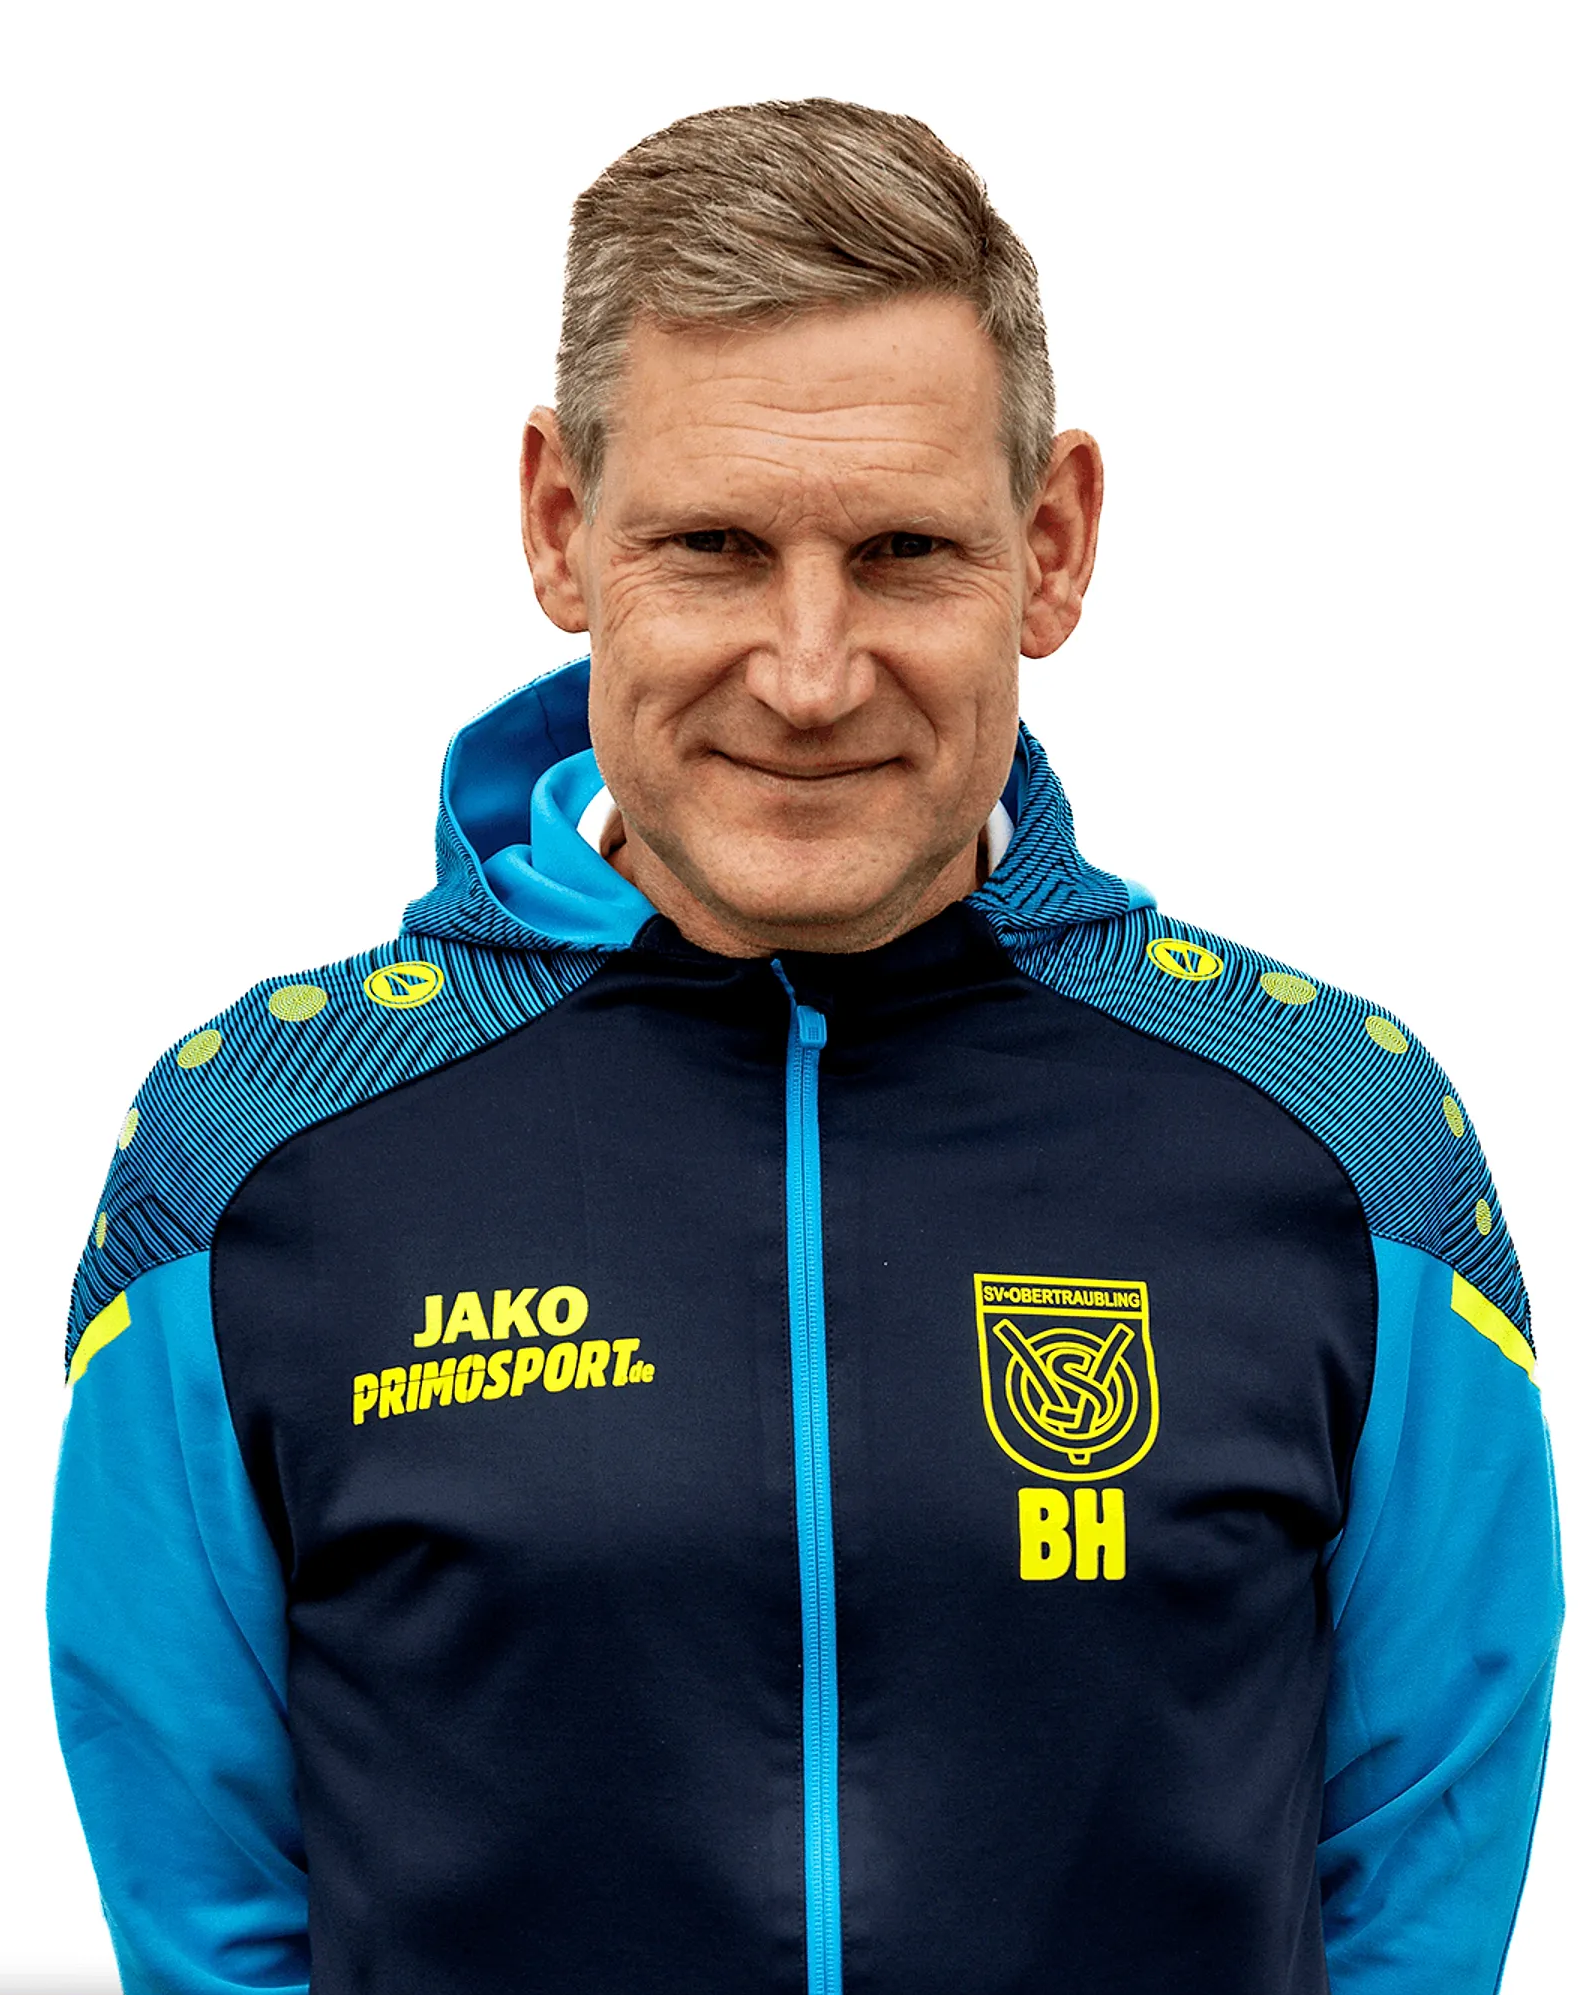
\includegraphics[width=\linewidth]{bilder/abteilungsleiter.png}
\end{minipage}

\vspace{1cm}

    \color{VereinsBlau} \textbf{SEHR GEEHRTE GÄSTE, FANS, LIEBE SPORTLERINNEN UND SPORTLER}

\vspace{0.5cm}
\normalsize \color{darkgray} 
\begin{doublespace}
	
im Namen der Fu\ss ballabteilung des SV Obertraubling heiße ich Sie zur neuen Saison 2025/2026 im
Sportzentrum Obertraubling recht herzlich willkommen.
Es ist viel passiert in den letzten Wochen und ich möchte Sie gerne mit ein paar Zeilen auf den aktuellen
Stand zu folgenden Themen bringen: das neue Trainerteam der 1. Mannschaft, die neue
„Eigenständigkeit“ der 2. Mannschaft sowie weitere Aktivitäten im Fußballbereich.
Zum Sportlichen:
Die 1. Mannschaft belegte in der vergangenen Saison mit einem SVO-Punkterekord (52) den 4.
Tabellenplatz. Gleichzeitig erreichte man damit die beste Punkte-Ausbeute der letzten 10 Jahre. Die
Abteilungsleitung, das Trainerteam und die Mannschaft waren mit dem Abschneiden jedoch nur
teilweise zufrieden, es hätte gerne einen oder zwei Plätze weiter nach oben gehen dürfen.
Die 2. Mannschaft belegte den 10. Tabellenplatz mit 25 Punkten und erfreulicherweise konnten wir
vom SVO den Großteil der Spieler im Saisonverlauf stellen. Während der Aufarbeitung der Saison hat
uns der Trainer der 1. Mannschaft, Florian Schmid, dann mitgeteilt, ab Sommer seine Zusammenarbeit
mit dem SVO zu beenden (O-Ton Bericht auf den nächsten Seiten).
Gleichzeitig sind wir von unserem SG Partner Neutraubling informiert worden, dass sich die Wege für
die 2. Mannschaft ab dem Sommer wieder trennen werden. Da in der kommenden Saison 2025/26
jahrgangsbedingt keine Spieler aus der A-Jugend in den Herrenbereich wechseln, standen die Zeichen
für den SVO zunächst einmal nicht sehr günstig.
Nach dem Motto „Jetzt erst recht“ setzte ein Netzwerk aus Spielern, Trainern, Betreuern und
Abteilungsleitung umgehend alle Hebel in Bewegung und so lassen sich für diese Saison einige
Neuzugänge vermelden. Die Vorstellung aller Neuzugänge erfolgt in den nächsten O-Ton Ausgaben. Auf der Suche nach einem Co-Trainer sind wir mit Luca Dippel fündig und einig geworden. Luca und
Marcel Scherl, unser Coach der 1. Mannschaft, kennen sich aus ihrer gemeinsamen Zeit beim SC
Regensburg.
Wir wünschen dem Duo gute Zusammenarbeit, viele Freude und Erfolg. Mit Johannes Koller haben wir
zudem einen Spielertrainer für unsere 2. Mannschaft gewonnen.
Jo kennt die jungen Spieler bestens und mit Sebastian Melzl und Franz „Golo“ Rieger hat er zwei
erfahrene Trainer an seiner Seite.
Erfreulicherweise sind die Spielgruppenleiter unserem Wunsch, die Heimspiele der 1. und 2. Mannschaft
hintereinander zu spielen, nachgekommen. So freuen wir uns, Ihnen ab sofort jeden Sonntag zwei Spiele
beim SVO anzubieten.
Für die nötige Verpflegung ist auch dieses Jahr wieder gesorgt, besuchen Sie unseren Stadionverkauf
und stärken Sie sich mit Kaffee, Kuchen und Erfrischungsgetränken.
Ich wünsche den jungen Mannschaften vom SVO viel Erfolg in der kommenden Saison, keine
Verletzungen und in allen Spielen das nötige Glück, um als Sieger vom Platz zu gehen.
Den Gästeteams und den mitgereisten Fans wünsche ich faire und spannende Spiele in unserer Leo-Graß-Arena.\\
\\
Mit sportlichen Grüßen\\
\\
Bernhard Hammermeier
\end{doublespace}